\documentclass{acm_proc_article-sp}
\usepackage{hyperref}
\usepackage[page,title]{appendix}
\usepackage{listings}
\usepackage{float}
\usepackage{amsmath}
\usepackage{varioref}
\pagenumbering{arabic}
\usepackage{moreverb}
\usepackage{url}
\usepackage{graphicx}
\restylefloat{table}
\usepackage{gensymb}
\usepackage{placeins}
\usepackage{adjustbox}
\usepackage{tabularx}
\usepackage{lipsum}

\usepackage[tableposition=top]{caption}
\begin{document}

\title{A Survey of Inertial Sensor Fusion}

\numberofauthors{1} 

\author{
\alignauthor Steven Paustian\\
       \affaddr{New Mexico Tech}\\
       \affaddr{801 Leroy Pl.}\\
       \affaddr{Socorro, New Mexico}\\
       \email{spaustia@nmt.edu}
}

\maketitle

\section{Introduction}

Mobile devices have become portable computers that support increased processing power and highly informative inertial sensors.  These sensors allow
for a level of context awareness that was not possible in previous devices.

Individual sensors are a wealth of information about the device's movement.  Unfortunately, single sensors are limited in the information they can provide about a device's inertial evolution due to inherent limitations.  By combining sensor measurements, we are able to gain a clearer picture of how the device is moving.  Algorithms to efficiently accomplish this task are consequently needed.  Currently, most sensor fusion algorithms are a variation of the Kalman Filter which is an recursive solution to the problem of combining sensor measurements.

In order to correctly interpret sensor measurements, we must know what limitations the data reflect.  In the following sections, we will discuss the different types of sensors found in most mobile devices, and what their constraints are, and how to efficiently combine sensor measurements into an optimal estimation of inertial movements.

\section{Accelerometer}

Mobile phone accelerometers work little differently than accelerometers used in other
devices or applications.\cite{brezmes2009activity}  Accelerometers measure linear acceleration of movement; this
stands in contrast to the gyroscope which measures angular rotational acceleration.
It is important to note that acceleration is defined as the change in
velocity over the change in time ($\frac{\Delta v}{\Delta t}$). To be more
specific, accelerometers measure deviation from freefall.  Therefore,
when the device is still or moving at a constant speed, the only measurement
displayed is that of gravity.  At that point this is the rate at which you are deviating from
falling.\cite{accell}

Modern accelerometers measure freefall deviation along three axises.  This allows 
for orientation and tilt sensing.  Using only the accelerometer, more than 20 human activities can be recognized
with reasonably high accuracy.\cite{wang2009framework}  There are several
significant limitations to mobile accelerometers, as will be discussed next.

\subsection{Limitations}
\subsubsection{Sampling Rate}
One limitation with the accelerometer is the sampling rate.  In order to retrieve accelerometer data,
the accelerometer is polled by the software.  Currently, there are no API's for Android
or Apple phones which allow software to control internal sampling rate.  
The hardware sampling rate is hardwired.\cite{brezmes2009activity}  While this may change
with future phones, currently, it is a limitation.

\subsubsection{Yaw}

Accelerometers are unable to process Yaw, which is the rotation of the device around an axis.  An example
of yaw is when a top is spinning on a level surface.  Movement is only happening about 1 axis, and that movement
is purely rotational in nature.  In order to recognize when a mobile device experiences yaw, one
must incorportate gyroscope, magnometer readings, or a second accelerometer.\cite{ashrafi2001relative}

\subsubsection{Noise}
As accelerometers measure all force working on an object, typical accelerometer
output includes more forces than a gravity vector.  Small forces disturb measurement.  This must
be combatted when using only accelerometer data by implementing some sort of filter; a low pass filter being popular.  When combining sensors, a Kalman filter can account for noise, as will be discussed later.

\subsubsection{Velocity \& Drift}

As the accelerometer readings show $\frac{\Delta v}{\Delta t}$ with regard to deviation from free-fall, velocity can be
found by approximating integration of these readings with respect to time:\cite{essl2007shamus}
 $$V(t) = \int_0^t V (t) dt \approx \displaystyle \sum \limits_{0}^t V (t)V_s$$.

When acceleration occurs faster than the sensor sampling rate can record, \textit{drift} becomes 
an issue that must be solved by combining gyroscopic data or including a second accelerometer.\cite{alves2003camera}

\section{Gyroscope}

Gyroscopes output the change in rotational velocity over time along three axises (angular velocity).
Angular velocity is the change in angular position over time.  Mathematically, this relationship is expressed
as $\frac{d\theta}{dt}$.\cite{gyro}
When combined with positional change, this is a very powerful tool.\cite{luinge2005measuring}

\subsection{Limitations}
\subsubsection{Angular Position \& Drift}

The raw measurements displayed by the gyroscope is the derivative of angular position: $\theta = \frac{d\theta}{dt}$.
To retrieve angular position, integration, or an approximation of integration, is necessary:
 $$\theta (t) = \int_0^t \theta (t) dt \approx \displaystyle \sum \limits_{0}^t \theta (t)T_s$$.\cite{gyro,luinge2005measuring}

Unfortunately, when the gyroscopic data changes at a quicker rate than the sampling
frequency reflects, an error will be introduced that increases with time known as \textit{drift}.\cite{luinge2005measuring} Mobile
gyroscopes are notorious for experiencing large drift values in short periods of time.  With unfiltered measurements, this author 
saw drifts up of up to 10 meters within 5 seconds of use.
In order to combat drift, we must increase sampling frequency as high as possible and
combine these readings with accelerometer data using a Kalman or Complementary Filter.\cite{gyro}  

%--------Comment!!!!
\begin{comment}
\section{Microphone}

Microphones on mobile devices convert sound waves around the phone into electrical signals
that can be interpreted by hardware and software.
Sound captured by the microphone on a mobile device can be a rich source
of information.\cite{lu2009soundsense}  There are three primary characteristics of
sound which can be analyzed: wavelength, frequency (pitch) and amplitude (volume).

While some sensors, such as accelerometer, report
1 specific piece of information regarding a system, the microphone 
contains many pieces of information.  For example, when a phone is dropped
it generates an impact sound.  This loudness of the sound can give insight into
the impact strength, while spectral information can tell us about the position
of impact.\cite{misra2008microphone}

Information gathered from this sensor are frequently used in conjunction
with other sensors to provide highly accurate insight about the user, environment, and social 
events.\cite{lu2009soundsense}  Much of the existing work on acoustic signal processing and classification can
be implemented on mobile platforms.\cite{lu2009soundsense}

One way microphones can be used to interpret events around them is through
framing.  

Unlike the camera, audio data from the microphone degrades in a graceful fashion.  The muffled sound 
heard when the device is in a pocket or backpack can still be used to gain valuable insight.

\subsection{Limitations}
Most of the difficulties related to interpreting information detected
by the microphone lie in the sheer volume and complexity of audio data. 

\subsubsection{Auditory Scene Analysis}
One of the primary limitations of sound analysis algorithms, is the difficulty
of algorithmically distinguishing specific sounds when there is noise.  For instance, it is
difficult to algorithmically distinguish a single person's voice from
the cacophany of sounds in a crowded party.

For other tasks, such as finding the musical key from a sequence of pitches,
there exist no robust algorithms.\cite{pauws2004musical}

\subsection{MARF}

The Modular Audio Recognization Framework (MARF), is a collection of algorithms for
sound, speech, and natural language processing creating a framework for feature extraction, preprocessing,
classification, etc.\cite{marf}  The framework is implemented in Java making it ideal to be
used in Android applications.
\end{comment}
%------------End Comments

\section{Magnetometer}

Magnetometers, commonly called "compass," measure the strength of magnetic fields around the device
along three axises.  When no magnetic interference is present near the device, the magnetometer will measure Earth's 
magnetic field.  When inteference is present, a robust algorithm must be applied to correctly interpret the data.\cite{psiaki1990three}

When a device experiences a constant magnetic field, even distorted, magnetometer readings will remain constant when corrected for noise.  
This makes them perfect candidates to correct drift inherit in gyroscopic readings.\cite{roetenberg2005compensation}

\subsection{Limitations}
\subsubsection{Magnetic Fields}

When in the presence of magnetic fields, magnometers readings are prone
to large and unpredictable errors.\cite{luinge2005measuring} Some of these magnetic fields
are created by the phone itself, mainly ferromagnetic materials that are present in the device's
battery, circuit boards, and component leads.  Calibration is necessary to offset the effects
of this noise.\cite{roetenberg2005compensation}

Sources of magnetic field reading contamination include the uneven magnetic field of the earth itself.  Our knowledge of which is inaccurate or insufficient in many locations.  Another source is ferrous metals.  Small deposits of these metals can influence the readings of our sensor at distances up to 100ft. \cite{psiaki1990three} Hence, even perfect measurements
by the sensor can lead to inaccurate conclusions by the algorithm which interprets them!\cite{psiaki1990three,roetenberg2005compensation}

\section{GPS}

The Global Positioning System (GPS) is a system of 27 satellites that provide location services to GPS receivers
that can see at least four satellites.  Many modern mobile devices include built-in GPS receivers.  When the receiver does not
have line of sight of at least four satellites, localization is provided by the service provider through triangulation of radio towers. 

\subsection{Limitations}
\subsubsection{Line of Sight}
GPS services work well when the device has line-of-sight to four or more satellites.  When it does not, localization services can sometimes be
provided through triangulation of the provider's cellular towers, though this makes for much less accurate location estimations.  Both Android and Apple API's provide access to both GPS and Network Localization
data, including (x,y) coordinates.\cite{krasner2003methods}

\subsubsection{Sampling rate}
Computing GPS location is relatively time and resource expensive for mobile devices.  Due to this, it is not possible to query
GPS coordinates at an exact instance in time.  Instead, localization is computed automatically by the device in regular intervals when available.
When working with GPS data, it is important to understand this limitation, as the data provided by the GPS sensor is termed "last known," and may not be accurate if the device is experiencing small movement before re-sampling. \cite{sencam}

\section{Camera}

Mobile phone cameras output two dimensional image arrays which can be processed as images.\cite{sencam}  Camera characteristics include resolution, focus type, and flash capabilities.  Cameras offer suplemental data that may be fused with IMU information to obtain 
better estimation of environmental variables.  The accuracy of position estimation from the camera is directly related to the quality of the images.\cite{alves2003camera}

To gain inertial measurements from camera images, one must apply a grid coordinate system to the image.  Then, landmark image characteristics in relation to the grid.  For the next frame, overlay the same grid system, and mark how image landmarks have changed coordinates.\cite{sencam}

\subsection{Limitations}
\subsubsection{Processing Resources}
Using the camera as an inertial sensor is highly resource intensive.  When using the camera as a sensor, one is essentially creating a video file for the length of the inertial measurements.  This can lead to huge memory costs as image quality is directly related to sensor reliability, and equal large CPU costs, as processing images is logic intensive.  Due to this, cameras in mobile devices are rarely well suited as sensors, as they are limited in battery life and processing power.\cite{alves2003camera}

\section{Sensor Fusion}

Sensor fusion is the process of integrating sensor information from several different sources into a unified interpretation of that data.
From this unification we can extract more meaningful, intelligent information.\cite{brooks1998multi}  This process is especially helpful when 
meauring changing external variables such as velocity, acceleration, angle of orientation and movement, and location as the inertial sensors
which are used to compute them suffer from bias error, noise and drift.\cite{sencam}\cite{klein2004sensor}

The vast majority of senor fusion algorithms are implemented using a variety of the Kalman Filter including the Discrete Kalman filter, Extended Kalman filter, and Unscented Kalman filter.\cite{brooks1998multi}   When processing resouces are valued, the Complementary filter is seen as a reasonable 
alternative.

\subsection{The Kalman Filter}

The Kalman Filter (KF) is a recursive solution to the problem of filting noisy measurements.  It provides an efficient computational 
way to estimate the past, present and future values outputed by an IMU.\cite{welch1995introduction}\cite{brooks1998multi} 

The Kalman Filter estimates the state of an IMU's readings, then it retrieves the actual measurements (with noise) that the
sensors are outputting.  We will refer to the estimates as \textit{time updates} and the retrieval of IMU data as \textit{measurement updates}.  \textit{Time updates} are predictions of what data should be, which are then corrected using \textit{measurement updates}.  Each set of \textit{measured updates} is
recursively applied to all prior and future estimations.  Two values, the Kalman gain and error covariance are used to correct the predictions.\cite{welch1995introduction}\cite{brooks1998multi}   After a
number of calculations, these values will approach a constant value as the errors within the system become more pronounced.  The Kalman gain and error covariance will offset the "noise" present in both sensor readings, allowing the software to better understand how device is moving or rotating. \cite{welch1995introduction}\cite{klein2004sensor,alves2003camera} Figure \ref{fig:kalman} depicts this process.


\begin{figure}[t]
\centering
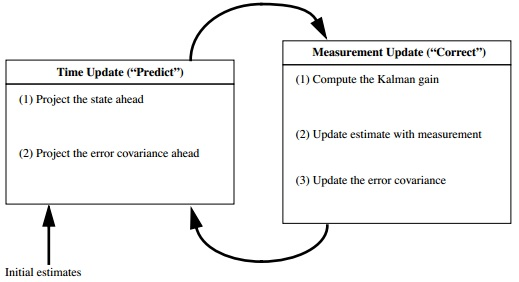
\includegraphics[width=90mm]{kalman.jpg}
\caption{An Overview of the Kalman filter control flow.}
\label{fig:kalman}
\end{figure}


Mathmatically, the Kalman Filter can be expressed as:

$$  \hat{X}_k = K_k \cdot Z_k + (1-K_k) \cdot \hat{X}_{x-1}  $$

Where $k$ subscripts are time states ($k$ = current time and $k-1$ = past measurement).  We are trying to find $\hat{X}_k$ which is the 
estimate of the signals.  $Z_k$ is the measurement values, and $K_k$ is the Kalman gain.  Because we know $Z_k$ and $\hat{X}_{k-1}$, we can calculate the Kalman gain using linear algebra.\cite{brooks1998multi} \cite{klein2004sensor}

Do accomplish this we let our time update be expressed as two equations: $$ x_k = Ax_{k-1} + Bu_k + w{k-1}$$ $$z_k = Hx_k + v_k $$

Here $x_k$ is the linear combination of its earlier value and noise.  $A, B$ and $H$ can be expressed as general form matrices or constant values, depending on the application.\cite{klein2004sensor}  Here we can assume they are constant.  We can estimate the mean $W_{k-1}$ and standard deviation $v_k$ using reasonable values.  The better these estimations, the better our final estimation.\cite{brooks1998multi} 

The measurement update can be expressed as the computation of the Kalman Gain ($K_k$),  $x_k$, and the error covariance ($P_k$):
$$ K_k = \frac{P_kH^T}{HP_kH^T+R}$$ $$ \hat{x}_k = \hat{x}_k + K_k(z_k-H\hat{x_k} $$ $$P_k = (I-K_kH)P_k $$

In order to find $Q$ and $R$ we need to estimate $X_0$ and $P_0$.  Once we have we can iterate according to Figure \ref{fig:kalman} where the Kalman gain is figured and a new estimation created based on that value and the measurements. \cite{welch1995introduction}

Note that this process only finds the corrected measurements of one sensor.  To combine additional sensors, we repeat the Kalman filter with another sensor's measurements, using the the optimal prediction of the previous sensor as the future prediction for the next sensor.\cite{klein2004sensor}\cite{welch1995introduction}

The main limitation with the Kalman sensor is that for it to function effectively, accurate initial readings are necessary.\cite{klein2004sensor}  In some circumstances this is not an issue e.g. measuring total angular rotation of the phone.\cite{brooks1998multi}   In other situations it is very important e.g. measuring angle of the phone with regards to some outside object; this requires that the initial offset be accurate.\cite{welch1995introduction}
\begin{table*}[t]
\centering
\begin{tabular}{ | l || c | c| c|c |}
 \hline
     \textbf{Actual Rotation ($\Theta$)} & $180\degree$  & $360\degree$ & $720\degree $ & $1080\degree$ \\ \hline\hline
    \textbf{Kalman Filter} & 182.34\degree &  366.84 \degree & 713.52\degree  & 1094.04\degree  \\ \hline
	\textit{\% Error: Kalman} & 1.3\% & 1.9\% & -0.9\% & 1.3\%   \\ \hline 
   \textbf{Complimentary Filter} & 175.14\degree & 348.8 \degree & 696.24\degree & 1037.9\degree \\  \hline
	\textit{\% Error: Complimentary} & -2.7\% & -3.1\% & -3.3\% & -3.9\% \\  \hline 
  \end{tabular}
 \\   \caption{Summary of filter readings.}
\label{ref:table}
\end{table*}
\subsection{The Complementary Filter}
While a full Kalman filter can be used to combine sensor data,
there exist two primary drawbacks towards it's use: its is both complex, and can be
difficult to implement.\cite{comp,mahony2005complementary}


The complimetary filter is in execution a steady-state Kalman filter that is both easy
to understand and implement.  Short term gyroscopic data is reliable and 
not susceptible to external forces; long term the 
information becomes increasingly error prone due to drift.\cite{mahony2005complementary}  Accelerometer data
does not suffer from drift, and is stable in the long term, but can be noisy.\cite{comp}  Therefore,
the complimentary filter serves to fuse the two data streams into a better estimation of device position.

The complimentary filter is straightforward in it's implementation and understanding.  Here is a simple equation to 
illustrate how to find angle of orientation of the device $\Theta_{new}$:  

$$ \Theta_{new} = (0.98)( \Theta_{old}+ \int_{t_a}^{t_b} GyroData \hspace{1 mm} dt )$$  $$ + (0.02)(AccelData)  $$

The variable HighPass is a constant defined as $\approx$ .98 and LowPass is defined as $\approx$ .02.  Therefore, the new angle of orientation, $\Theta$, can be found using 98\% of the change in angle as reported by the gryoscope offset by the old angle, plus 2\% of the acceleration data to
account for the gyroscopic drift.\cite{comp}  This is much simpler than a Kalman filter once the correct weights have been found using trial and error.



\begin{comment}
\section{Energy Efficiency}

A capable technique to reduce power consumption when using multiple sensors
is to "cycle" them.  For example, when attempting to recognize a user's location,
one may wish to cycle WiFi off until the person has stopped moving.  Then once movement has stopped,
WiFi could be turned on and GPS turned off.  This cycling has proven to significantly reduce
power consumption on mobile devices.\cite{wang2009framework}
\end{comment}

\section{Implementation}
The author implemented a Kalman filter and Complementary filter on his HTC One X in Java using the Android SDK.  Sensor fusion was performed on Accelerometer, Gyroscope, and Magnetometer to find the final angular position ($\Theta$) of the phone after spinning around an axis.  The camera was not used as the implementation of inertial readings from images is beyond this author's skill; nor was GPS data as it isn't applicable to rotational measurements.

 The phone was attached (taped) to a drill bit in a drill and spun at low velocity for a varying number of rotations as seen in Figure \ref{fig:drill} .  The Kalman and Complementary Filter resulted in similar angle readings, though there were differences. The percentage error and final $\Theta$ readings are surmised in the Table \ref{ref:table} .  While this experiment may seem over-simple, finding a device's angle is surprisingly difficult, and an ongoing source of research in robotics and mobile devices.\cite{barshan1995inertial}

\begin{figure}[ht]
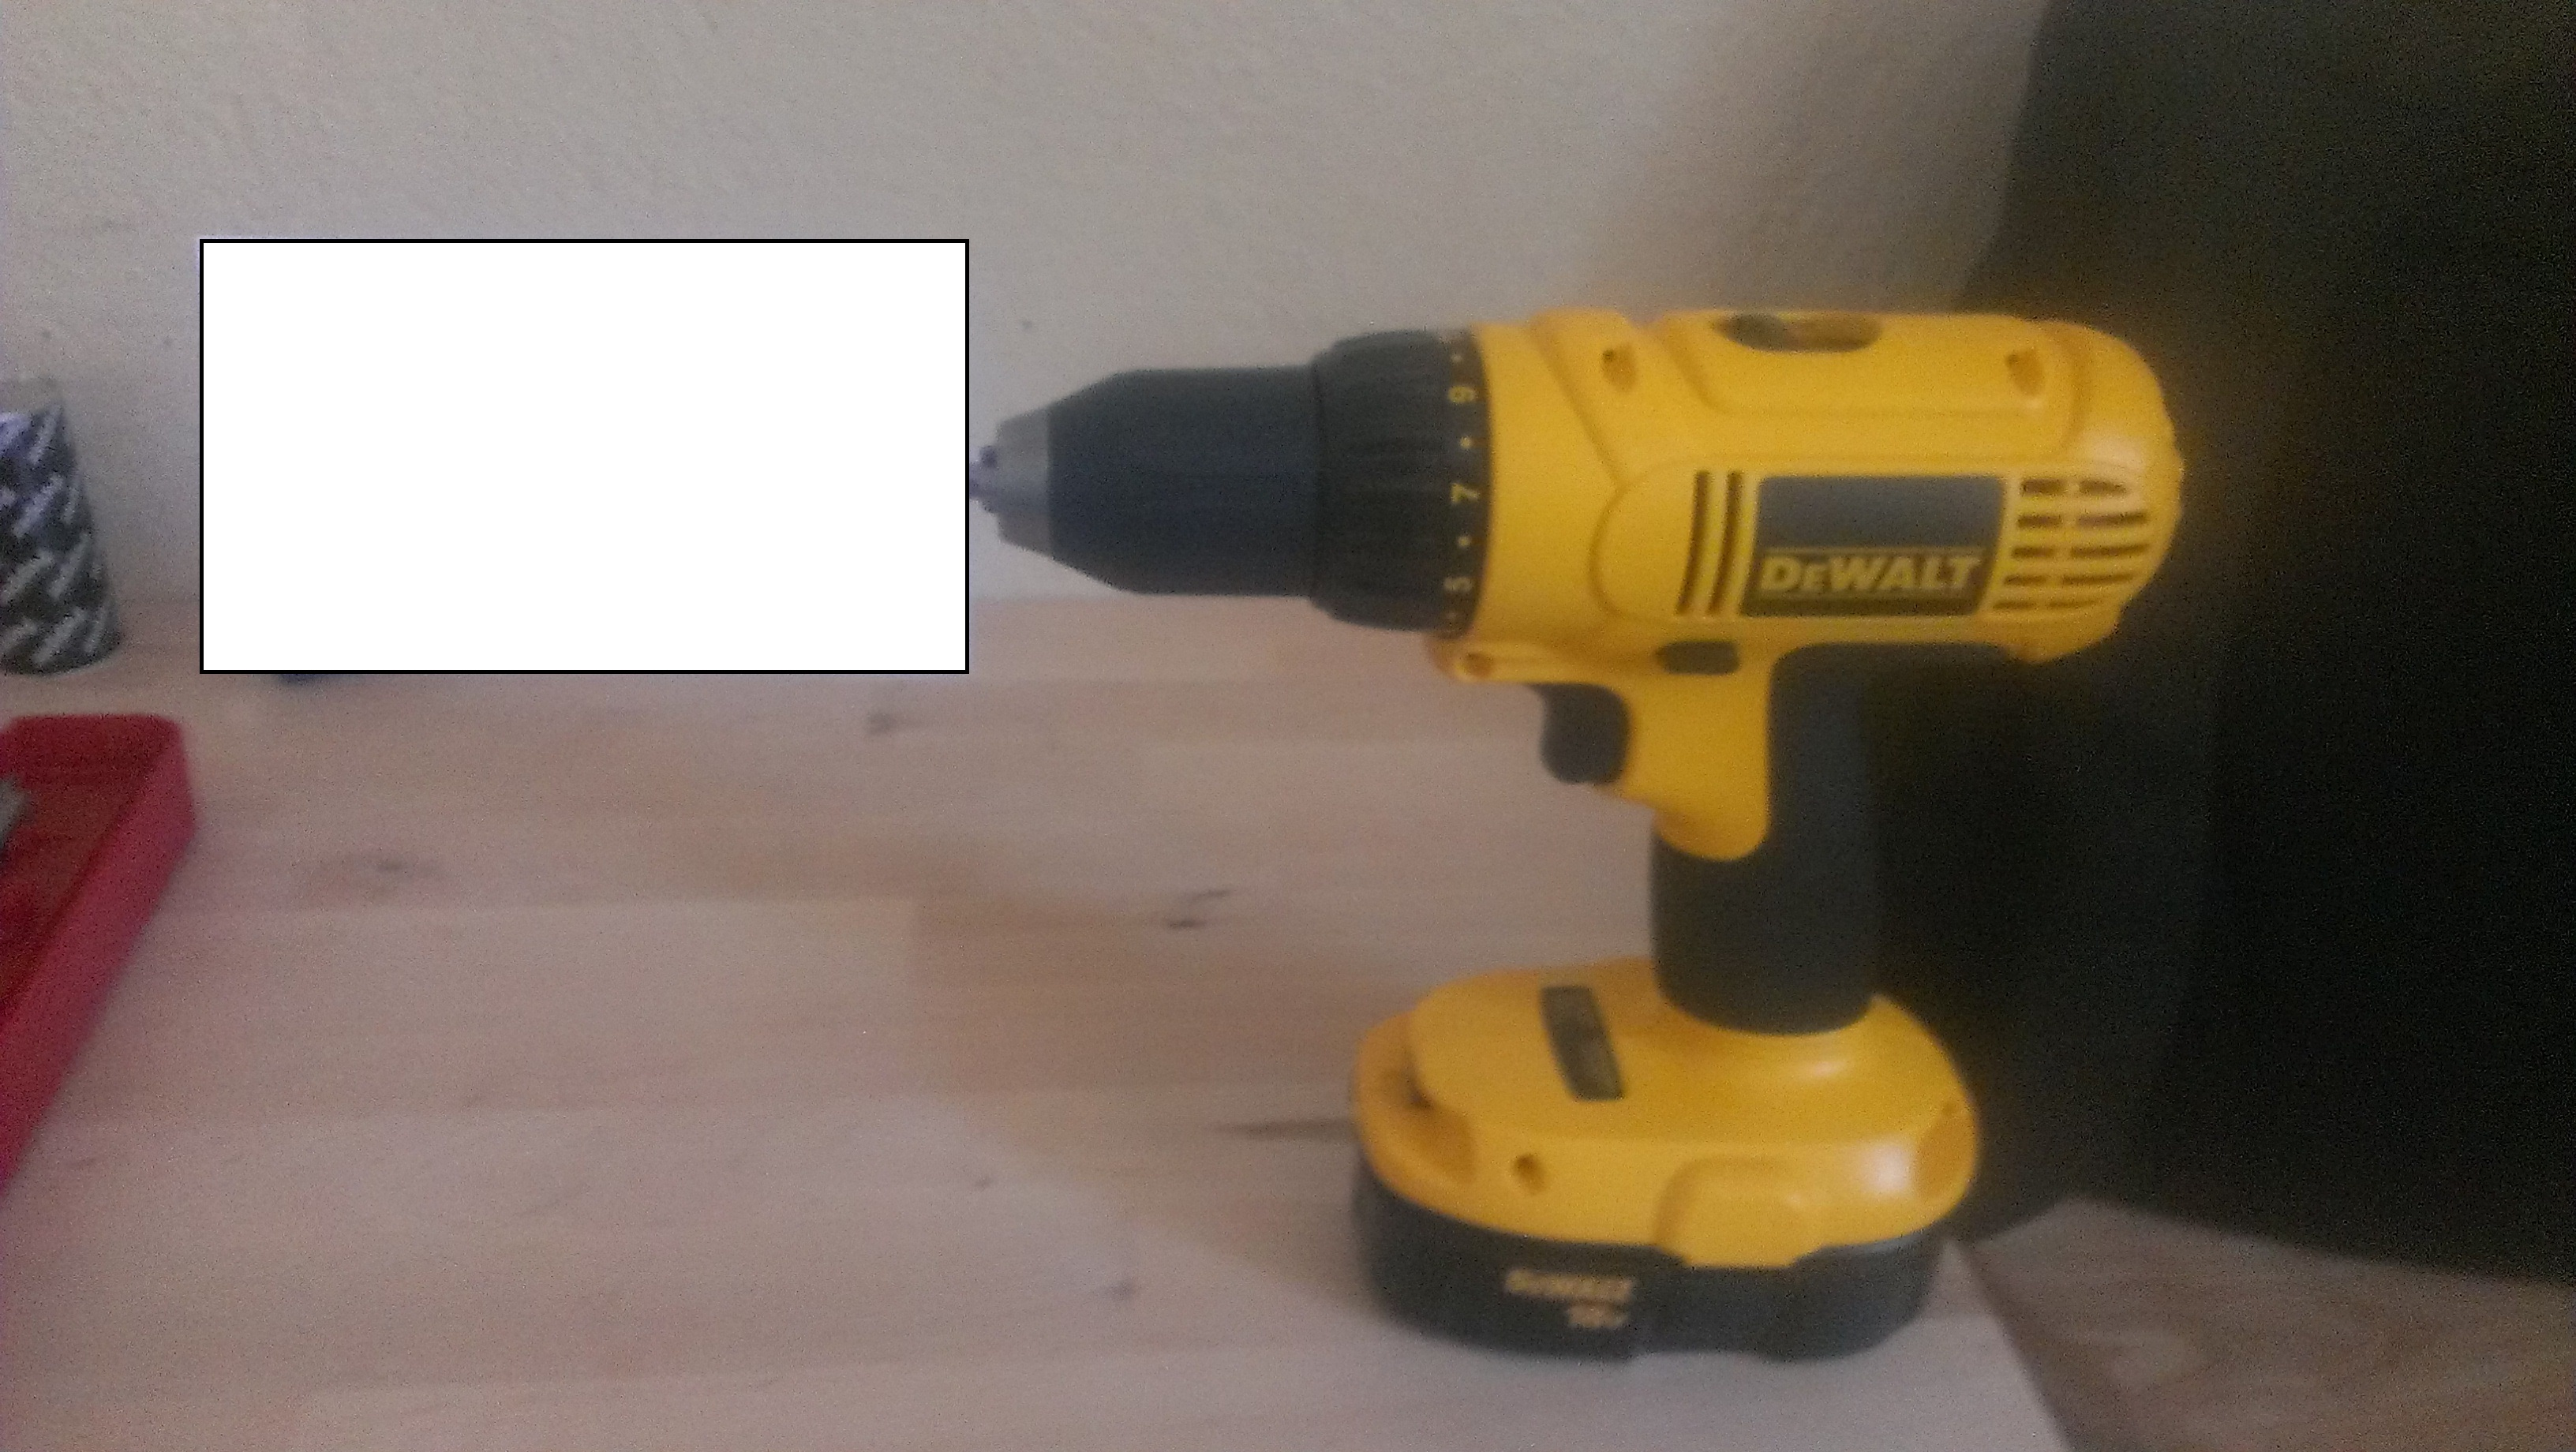
\includegraphics[width=70mm, height=70mm]{drill.jpg}
\caption{Experimental Setup.  Note that the phone was placed where the blank space is seen, as to obtain a picture of the device the phone's camera was needed.}
\label{fig:drill}
\end{figure}
 
It is interesting to note that the complementary filter's error increases as the time spend rotating increases.  The time spent rotating and the total rotations made no difference in the Kalman Filter's estimation.  This is a clearly an advantage of the Kalman Filter.

If accurate readings are required for long periods of time, the Kalman filter is superior.  When individual measurements not dependent upon previous estimations are adequate, the complimentary filter may be used to good effect.

\section{Conclusion}

In order to gain a clear picture of a mobile device's inertial movements, a Kalman filter or some variation of it is required.  As can be seen in Table \ref{ref:table}, a Kalman filter efficiently combines the measurements of multiple sensors into a significantly more accurate picture of a device's movement than can be gained by using 1 sensor alone.

\begin{appendices}

\end{appendices}

\bibliographystyle{abbrv}
\bibliography{final}

\end{document}

